\documentclass[12pt, titlepage, a4paper]{article}
\usepackage[utf8x]{inputenc}
\usepackage[T1]{fontenc}
\usepackage{graphicx}
\title{Assignment 2: Use Case Modelling}
\date{\today}
\author{Marijan Svalina \\ Damir Jelić}

\begin{document}

\maketitle 

\setcounter{section}{2}
\subsection{Identification}

\begin{description}
    \item[Actors:] \hfil
    \begin{itemize}
    \item
        Customer
        \begin{description}
            \item[]Customer is an actor who is registered on the web page and is a potential buyer, 
            he can use the system to browse through the available 
            property list an place purchase orders. 
        \end{description}
    \item
        Seller
        \begin{description}
            \item[]Seller is an actor who is deals with the purchase orders and confirms them,
		    he also manages the web page and writes promotional material.
        \end{description}
    \end{itemize}

    \item[Use cases:] \hfil
    \begin{itemize}
    \item
        \begin{description}
            \item[Name:]Buy record online 
            \item[Initiator:]Customer
            \item[Goal:]Buy a record at the online shop 
            \begin{enumerate}
                \item Customer browses the web page for a record
                \item Customer decides which record(s) to buy
                \item Customer places the record(s) in the basket
                \item The system sends the order to the seller for processing
                \item The seller confirms the order to the system
                \item The system sends the confirmation with the invoice to the customer
            \end{enumerate}
            \item[Extensions:] \hfil
            \begin{enumerate}
                \item Requested record is out of stock
                \begin{enumerate}
                    \item System allows customer to choose different record
                    \item Resume at 1
                \end{enumerate}
            \end{enumerate}
        \end{description}

    \item
        \begin{description}
            \item[Name:]Listen sample online 
            \item[Initiator:]Customer
            \item[Goal:]Listen to a record before buying it
            \begin{enumerate}
                \item Customer browses the web page for a record
                \item Customer chooses to listen to a sample from the record
                \item System provides an audio stream to the customer
            \end{enumerate}
    	    \item[Extensions:] \hfil
	    \begin{enumerate}
		\item Customers browser doesn't support audio codec
		\begin{enumerate}
			\item System prints error message
		\end{enumerate}
	    \end{enumerate}
        \end{description}

    \item
        \begin{description}
            \item[Name:]Send promotional e-mail 
            \item[Initiator:]Seller
            \item[Goal:]Send some promotional material to customers 
	    \begin{enumerate}
		\item Seller writes newsletter
		\item Seller requests top selling records from system
		\item Seller attaches record list to newsletter
		\item Seller gives the newsletter to the system
		\item System sends the newsletter to the customers
		\end{enumerate}
        \end{description}

    \item 
        \begin{description}
            \item[Name:]Search online store
		    \item[Initiator:]Customer
		    \item[Goal:]Getting quick access to exact record\dots
		    \begin{enumerate}
		    	\item Customer writes keyword in search field
			\item Customer starts search
			\item System delivers search results
		    \end{enumerate}
        \end{description}
    \item 
        \begin{description}
		\item[Name:]Rate a record 
		\item[Initiator:]Customer 
		\item[Goal:]Contribute back to other customers with personal review 
			\begin{enumerate}
			\item Customer browses the web pages
			\item Customer rates the record and writes a review
			\item System saves reviews and display it under the record page
			\end{enumerate}
        \end{description}
    \end{itemize}
\end{description}

\subsection{Diagram}
    \begin{center}
        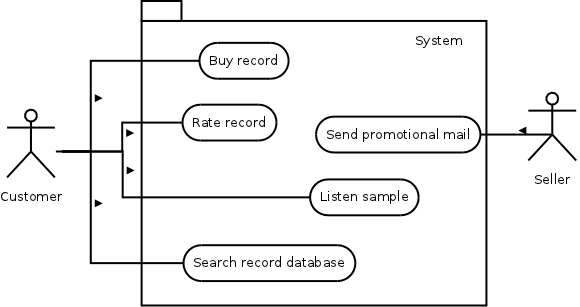
\includegraphics[scale=0.47]{lab2.png}
    \end{center}
\end{document}
